\documentclass{book}

\usepackage{etoolbox}

\makeatletter
\def\subtitle#1{\gdef\@subtitle{#1}}
\patchcmd\maketitle
  {{\LARGE \@title \par}}
  {{\LARGE \@title \par}%
   \vskip 1.5em
   {\Large \@subtitle \par}}
\makeatother

\usepackage[utf8x]{inputenc}
\usepackage{amsmath,mathtools,bbm}
\usepackage{amsfonts}
\usepackage{amssymb}
\usepackage{graphicx}
\usepackage{appendix}
\usepackage{enumitem}
\usepackage{bm}
\usepackage{multicol}
\usepackage{geometry}
\usepackage{colortbl}
\usepackage{changepage}
\usepackage{color}
\usepackage{mathrsfs}
\usepackage{bigints}
\usepackage{pdflscape}
\usepackage{adjustbox}
\usepackage{tocloft}
\usepackage{lscape}
\usepackage[dvipsnames]{xcolor}
\usepackage[colorlinks=true,
            linkcolor=blue,
            urlcolor=blue,
            citecolor=blue]{hyperref}

\sloppy
\usepackage{tikz, lipsum}% http://ctan.org/pkg/{pgf,lipsum}
\newcommand*{\chapnumfont}{\normalfont\sffamily\huge\bfseries}
\newcommand*{\printchapternum}{
  
\begin{tikzpicture}
    \draw[fill,color=gray75] (0,0) rectangle (2cm,2cm);
    \draw[color=white] (1cm,1cm) node { \chapnumfont\thechapter };
  \end{tikzpicture}
}
\newcommand*{\chaptitlefont}{\normalfont\sffamily\Huge\bfseries}
\newcommand*{\printchaptertitle}[1]{\flushright\chaptitlefont#1}

\makeatletter
% \@makechapterhead prints regular chapter heading.
% Taken directly from report.cls and modified.
\def\@makechapterhead#1{%
  \vspace*{50\p@}%
  {\parindent \z@ \raggedleft
    \ifnum \c@secnumdepth >\m@ne
        \printchapternum
        \par\nobreak
        \vskip 20\p@
    \fi
    \interlinepenalty\@M
    \printchaptertitle{#1}\par\nobreak
    \vskip 40\p@
  }}
% \@makeschapterhead prints starred chapter heading.
% Taken directly from report.cls and modified.
\def\@makeschapterhead#1{%
  \vspace*{50\p@}%
  {\parindent \z@ \raggedleft
    \interlinepenalty\@M
    \printchaptertitle{#1}\par\nobreak
    \vskip 40\p@
  }}
\makeatother

\makeatletter\@addtoreset{chapter}{part}\makeatother%

\renewcommand\contentsname{}

\definecolor{gray75}{gray}{0.75}

\title{\Huge \bfseries\sffamily Diffusing Ideas}
\subtitle{\Large \bfseries\sffamily \color{gray75} Software, noise and building mathematical toys}
\author{\bfseries\sffamily Robert J. Hardwick}
\date{\today}
\begin{document}
\maketitle
\frontmatter

\chapter*{Introduction}

\emph{Diffusing Ideas} is a book of research exploration and software development which I have written for the interest of mathematically-inclined programmers and computational scientists. It's the output of many interrelated projects over several years which have sought to generalise the computational mathematics of simulating, statistically inferring, manipulating and automatically controlling stochastic phenomena as far as possible. 

The book accompanies a lot of new open-source scientific software, written predominantly in \href{https://www.python.org/}{Python} and \href{https://go.dev/}{Go}. A major motivation for creating these new tools is to prepare a foundation of code from which to develop new and more complex applications. I also hope that the resulting framework will enable anyone to explore and study new phenomena effectively, regardless of their scientific background.

The need to properly test all this software has also provided a wonderful excuse to study and play with an extensive range of mathematical toy models. I've chosen these models based on my broad background of interests, but also to illustrate the remarkable cross-disciplinary applicability of stochastic processes. However, it's often true that mathematical formalities can obscure the computations that a programmer must implement. So, while I've tried to be as ambitious as possible with the level of technical sophistication in these models, I've also tried to write the expressions in a computer-friendly way.\footnote{E.g., more `matrices' and less `operators'.}

A quick note on the code: any software that I describe in this book (including the \href{https://github.com/umbralcalc/diffusing-ideas}{software which compiles the book itself}) will always be shared under a \href{https://opensource.org/licenses/MIT}{MIT License} in a public Git repository.\footnote{The repositories will always be somewhere on this list: \href{https://github.com/umbralcalc?tab=repositories}{https://github.com/umbralcalc?tab=repositories}.} Forking these repositories and submitting pull requests for new features or applications is strongly encouraged too, though I apologise in advance if I don't follow these up very quickly as all of this work has to be conducted independently in my free time, outside of work hours.

No quest would be complete without a guide, so to end this introduction, I think it makes the most sense to outline the key milestones and their motivations within the context of the overall research project. My core aims, which comprise the four major parts of this book, are answers to the following set of interdependent research questions:

\begin{enumerate}[leftmargin=2.5\parindent] 
\item[{\bfseries\sffamily Part 1.}]{How do we simulate a general set of stochastic phenomena?}
\item[{\bfseries\sffamily Part 2.}]{How do we then learn/identify the answer to {\bfseries\sffamily Part 1} from real-world data?}
\item[{\bfseries\sffamily Part 3.}]{How do we simulate a general set of control policies to interact with the answer to {\bfseries\sffamily Part 1}?}
\item[{\bfseries\sffamily Part 4.}]{How do we then optimise the answer to {\bfseries\sffamily Part 3} to achieve a specified control objective?} 
\end{enumerate}



\chapter*{Table of contents}
\vspace*{-3cm}
{\sffamily \tableofcontents}
\mainmatter


\part*{{\sffamily {\color{gray75} Part 1.} How do we simulate a general set of stochastic phenomena?}}


\chapter{\sffamily Building a generalised simulator}

{\bfseries\sffamily Concept.} To design and build a generalised simulation engine that is able to generate samples from a `Pokédex' of possible stochastic processes that a researcher might encounter. A `Pokédex' here is just my fanciful description for a very general class of multidimensional stochastic processes that pop up everywhere in taming the mathematical wilds of real-world phenomena, and which also leads to a name for the software itself: the `stochadex'. With such a thing pre-built and self-contained, it can become the basis upon which to build generalised software solutions for a lot of different problems. For the mathematically-inclined, this chapter will require the introduction of a new formalism which we shall refer back to throughout the book. For the programmers, the public Git repository for the code that is described in this chapter can be found here: \href{https://github.com/umbralcalc/stochadex}{https://github.com/umbralcalc/stochadex}.

\section{\sffamily Computational formalism}

Before we dive into the software and some examples, we need to mathematically define the general computational approach that we're going to take in order to be able to describe as general a set of stochastic phenomena as possible. From experience, it seems reasonable to start by writing down the following formula which describes iterating some arbitrary process forward in time (by one finite step) and adding a new row each to some matrix $X' \rightarrow X$
%%
\begin{align}
X^{i}_{{\sf t}+1} &= F^{i}_{{\sf t}+1}(X',{\sf t}) \,, \label{eq:x-step-def}
\end{align}
%%
where: $i$ is an index for the dimensions of the `state' space; ${\sf t}$ is the current time index for either a discrete-time process or some discrete approximation to a continuous-time process; $X$ is the next version of $X'$ after one timestep (and hence one new row has been added); and $F^i_{{\sf t}+1}(X',{\sf t})$ as the latest element of an arbitrary matrix-valued function. As we shall discuss shortly, $F^i_{{\sf t}+1}(X',{\sf t})$ may represent not just operations on deterministic variables, but also on stochastic ones. There is also no requirement for the function to be continuous.

So the basic computational idea here is to iterate the matrix $X$ forward in time by a row, and use its previous version $X'$ as an entire matrix input into a function which populates the elements of its latest rows. Pretty simple! But why go to all this trouble of storing matrix inputs for previous values of the same process? It's true that this is mostly redundant for \emph{Markovian} phenomena, i.e., processes where their only memory of their history is the most recent value they took. However, for a large class of stochastic processes a full memory\footnote{Or memory at least within some window.} of past values is essential to consistently construct the sample paths moving forward. This is true in particular for \emph{non-Markovian} phenomena, where the latest values don't just depend on the immediately previous ones but can depend on values which occured much earlier in the process as well.

For more complex physical models and integrators, the distinct notions of `numerical timestep' and `total elapsed continuous time' will crop up quite frequently. Hence, before moving on further details, it will be important to define the total elapsed time variable $t({\sf t})$ for processes which are defined in continuous time. Assuming that we have already defined some function $\delta t({\sf t})$ which returns the specific change in continuous time that corresponds to the step ${\sf t}-1 \rightarrow {\sf t}$, we will always be able to compute the total elapsed time through the relation
%%
\begin{align}
t({\sf t}) &= \sum^{{\sf t}}_{{\sf t}'=0}\delta t({\sf t}') \,.
\end{align}
%%
This seems a lot of effort, no? Well it's important to remember that our steps in continuous time may not be constant, so by defining the $\delta t({\sf t})$ function and summing over it we can enable this flexibility in the computation.

So, now that we've mathematically defined a really general notion of iterating the stochastic process forward in time, it makes sense to discuss some simple examples. For instance, it is frequently possible to split $F$ up into deteministic (denoted $D$) and stochastic (denoted $S$) matrix-valued functions like so
%%
\begin{align}
& F^{i}_{{\sf t}+1}(X',{\sf t}) = D^{i}_{{\sf t}+1}(X',{\sf t}) + S^{i}_{{\sf t}+1}(X',{\sf t}) \,.
\end{align}
%%
In the case of stochastic processes with continuous sample paths, it's also nearly always the case with mathematical models of real-world systems that the deterministic part will at least contain the term $D^{i}_{{\sf t}+1}(X',{\sf t}) = X^i_{\sf t}$ because the overall system is described by some stochastic differential equation. This is not a really requirement in our general formalism, however.

What about the stochastic term? For example, if we wanted to consider a \emph{Wiener process noise}, we can define $W^i_{{\sf t}}$ is a sample from a Wiener process for each of the state dimensions indexed by $i$ and our formalism becomes
%%
\begin{align}
& S^{i}_{{\sf t}+1}(X',{\sf t}) = W^i_{{\sf t}+1}-W^i_{\sf t} \label{eq:wiener}\,.
\end{align}
%%
One draws the increments $W^i_{{\sf t}+1}-W^i_{\sf t}$ from a normal distribution with a mean of $0$ and a variance equal to the length of continuous time that the step corresponded to $\delta t({\sf t}+1)$, i.e., the probability density $P^i_{{\sf t}+1}(x)$ of the increments $x^i=W^i_{{\sf t}+1}-W^i_{\sf t}$ is
%%
\begin{align}
P^i_{{\sf t}+1}(x) &= {\sf NormalPDF}[x^i;0,\delta t({\sf t}+1)] \,.
\end{align}
%%
Note that for state spaces with dimensions $>1$, we could also allow for non-trivial cross-correlations between the noises in each dimension.

In another example, to model \emph{geometric Brownian motion noise} we would simply have to multiply $X^i_{\sf t}$ to the Wiener process like so
%%
\begin{align}
& S^{i}_{{\sf t}+1}(X',{\sf t}) = X^i_{\sf t}(W^i_{{\sf t}+1}-W^i_{\sf t})\label{eq:gbm} \,.
\end{align}
%%
Here we have implicitly adopted the Itô interpretation to describe this stochastic integration. Given a carefully-defined integration scheme other interpretations of the noise would also be possible with our formalism too, e.g., Stratonovich\footnote{Which would implictly give $S^{i}_{{\sf t}+1}(X',{\sf t}) = (X^i_{{\sf t}+1}+X^i_{\sf t})(W^i_{{\sf t}+1}-W^i_{\sf t}) / 2$ for Eq.~(\ref{eq:gbm}).} or others within the more general `$\alpha$-family'~\cite{van1992stochastic,risken1996fokker,rog-will-2000}.

We can imagine even more general processes that are still Markovian. One example of these in a single-dimension state space would be
%%
\begin{align}
S^0_{{\sf t}+1}(X',{\sf t}) &= g[W^0_{{\sf t}+1},t({\sf t}+1)]-g[W^0_{\sf t}, t({\sf t})] \\
&= \bigg[ \frac{\partial g}{\partial t} + \frac{1}{2}\frac{\partial^2 g}{\partial x^2} \bigg] \delta t ({\sf t}+1) + \frac{\partial g}{\partial x} (W^0_{{\sf t}+1}-W^0_{\sf t}) \label{eq:general-wiener}\,,
\end{align}
%%
where $g(x,t)$ is some continuous function of its arguments which has been expanded out with Itô's Lemma on the second line. Note also that the computations in Eq.~(\ref{eq:general-wiener}) could be performed with numerical derivatives in principle if the function were extremely complicated.

Let's now look at a more complicated type of noise. For example, \emph{fractional Brownian motion} $[B_{H}]_{\sf t}$ with Hurst exponent $H$. Following Ref.~\cite{decreusefond1999stochastic}, we can simulate this process in one of our state space dimensions by modifying a standard Wiener process like so
%%
\begin{align}
S^{0}_{{\sf t}+1}(X',{\sf t}) &= \frac{(W^0_{{\sf t}+1} - W^0_{\sf t})}{\delta t({\sf t}+1)}\int^{t({\sf t}+1)}_{t({\sf t})}{\rm d}t' \frac{(t'-t)^{H-\frac{1}{2}}}{\Gamma (H+\frac{1}{2})} {}_2F_1 \bigg( H-\frac{1}{2};\frac{1}{2}-H;H+\frac{1}{2};1-\frac{t'}{t}\bigg) \label{eq:fbm} \,,
\end{align}
%%
where $S^{0}_{{\sf t}+1}(X',{\sf t})=[B_{H}]_{{\sf t}+1}-[B_{H}]_{{\sf t}}$. The integral in Eq.~(\ref{eq:fbm}) can be approximated using an appropriate numerical procedure (like the trapezium rule). In the expression above ${}_2F_1$ and $\Gamma$ are the ordinary hypergeometric and gamma functions, respectively.

So far we have mostly been discussing noises with continuous sample paths, but we can easily adapt our computation to discontinuous sample paths as well. For instance, \emph{Poisson process noises} would generally take the form
%%
\begin{align}
S^{i}_{{\sf t}+1}(X',{\sf t}) &= [N_{\lambda}]^i_{{\sf t}+1}-[N_{\lambda}]^i_{\sf t}\,,
\end{align}
%%
where $[N_{\lambda}]^i_{\sf t}$ is a sample from a Poisson process with rate $\lambda$. One can think of this process as counting the number of events which have occured up to the given interval of time, where the intervals between each succesive event are exponentially distributed with mean $1/\lambda$. Such a simple counting process could be simulated exactly by explicitly setting a newly-drawn exponential variate to the next continuous time jump ${\delta t}({\sf t}+1)$ and iterating the counter. Other exact methods exist to handle more complicated processes involving more than one type of `event', such as the Gillespie algorithm~\cite{gillespie1977exact} --- though these techniques are not always be applicable in every situation.

Is using step size variation always possible? If we consider a \emph{time-inhomogeneous Poisson process noise}, which would generally take the form
%%
\begin{align}
S^{i}_{{\sf t}+1}(X',{\sf t}) &= [N_{\lambda ({\sf t}+1)}]^i_{{\sf t}+1}-[N_{\lambda ({\sf t})}]^i_{\sf t}\,,
\end{align}
%%
the rate $\lambda ({\sf t})$ has become a deterministically-varying function in time. In this instance, it likely not be accurate to simulate this process by drawing exponential intervals with a mean of $1/\lambda ({\sf t})$ because this mean could have changed by the end of the interval which was drawn. An alternative approach (which is more generally capable of simulating jump processes but is an approximation) first uses a small time interval $\tau$ such that the most likely thing to happen in this period is nothing, and then the probability of the event occuring is simply given by
%%
\begin{align}
p({\sf event}) &= \frac{\lambda ({\sf t})}{\lambda ({\sf t}) + \frac{1}{\tau}} \label{eq:rejection}\,.
\end{align}
%%
This idea can be applied to phenomena with an arbitrary number of events and works well as a generalised approach to event-based simulation, though its main limitation is worth remembering; in order to make the approximation good, $\tau$ often must be quite small and hence our simulator must churn through a lot of steps. From now on we'll refer to this well-known technique as the \emph{rejection method}.

There are a few extensions to the simple Poisson process that introduce additional stochastic processes. \emph{Cox (doubly-stochastic) processes}, for instance, are basically where we replace the time-dependent rate $\lambda ({\sf t})$ with independent samples from some other stochastic process $\Lambda ({\sf t})$. For example, a Neyman-Scott process~\cite{neyman1958statistical} can be mapped as a special case of this because it uses a Poisson process on top of another Poisson process to create maps of spatially-distributed points. In our formalism, a two-state implementation of the Cox process noise would look like
%%
\begin{align}
S^{0}_{{\sf t}+1}(X',{\sf t}) &= \Lambda ({\sf t}+1) \\
S^{1}_{{\sf t}+1}(X',{\sf t}) &= [N_{S^{0}_{{\sf t}+1}}]^i_{{\sf t}+1}-[N_{S^{0}_{{\sf t}}}]^i_{\sf t}\,.
\end{align}
%%
Another extension is \emph{compound Poisson process noise}, where it's the count values $[N_{\lambda}]^i_{\sf t}$ which are replaced by independent samples $[J_{\lambda}]^i_{\sf t}$ from another probability distribution, i.e.,
%%
\begin{align}
S^{i}_{{\sf t}+1}(X',{\sf t}) &= [J_{\lambda}]^i_{{\sf t}+1}-[J_{\lambda}]^i_{\sf t}\,.
\end{align}
%%
Note that the rejection method of Eq.~(\ref{eq:rejection}) can be employed effectively to simulate any of these extensions as long as a sufficiently small $\tau$ is chosen.

All of the examples we have discussed so far are Markovian. Given that we have explicitly constructed the formalism to handle non-Markovian phenomena as well, it would be worthwhile going some examples of this kind of process too. \emph{Self-exciting process noises} would generally take the form
%%
\begin{align}
S^{0}_{{\sf t}+1}(X',{\sf t}) &= {\cal I}_{{\sf t}+1} (X',{\sf t}) \\
S^{1}_{{\sf t}+1}(X',{\sf t}) &= [N_{S^{0}_{{\sf t}+1}}]^i_{{\sf t}+1}-[N_{S^{0}_{{\sf t}}}]^i_{\sf t} \,,
\end{align}
%%
where the stochastic rate ${\cal I}_{{\sf t}+1} (X',{\sf t})$ now depends on the history explicitly. Amongst other potential inputs we can see, e.g., Hawkes processes~\cite{hawkes1971spectra} as an example of above by substituting 
%%
\begin{align}
{\cal I}_{{\sf t}+1} (X',{\sf t}) &= \mu + \sum^{{\sf t}}_{{\sf t}'=0}\gamma [t({\sf t})-t({\sf t}')](S^{1}_{{\sf t}'}-S^{1}_{{\sf t}'-1}) \,,
\end{align}
%%
where $\gamma$ is the `exciting kernel' and $\mu$ is some constant background rate. 

Note that this idea of integration kernels could also be applied back to our Wiener process. For example, another type of non-Markovian phenomenon that frequently arises across physical and life systems integrates the Wiener process history like so
%%
\begin{align}
S^{0}_{{\sf t}+1}(X',{\sf t}) &= W^0_{{\sf t}+1}-W^0_{\sf t}\\
S^{1}_{{\sf t}+1}(X',{\sf t}) &= \frac{1}{T}\sum^{{\sf t}}_{{\sf t}'=0}e^{-\frac{t({\sf t})-t({\sf t}')}{T}} (S^{0}_{{\sf t}'}-S^{0}_{{\sf t}'-1}) \,,
\end{align}
%%
where $T$ is some decay coefficient which quantifies the length of memory in continuous time.

So we've introduced the basic elements of our computational formalism and demonstrated how flexible the approach can be in simulating just about any stochastic phenomenon imaginable. Before progressing to algorithm design, it will be helpful to discuss some useful concepts that should enable us analyse the system later on in the book.

\section{\sffamily Useful probabilistic concepts}

The general stochastic process that we defined with Eq.~(\ref{eq:x-step-def}) also has an implicit \emph{master equation} associated to it which fully describes the time evolution of the \emph{probability density function} $P_{{\sf t}+1}(x)$ of the most recent matrix row $x=X_{{\sf t}+1}$ at time ${\sf t}$. This can be written as
%%
\begin{align}
P_{{\sf t}+1}(x) &= \frac{1}{{\sf t}}\sum_{{\sf t}'=0}^{{\sf t}}\int_{\omega_{{\sf t}'}}{\rm d}x' P_{{\sf t}'}(x') P_{({\sf t}+1){\sf t}'}(x\vert x') \label{eq:master-x-cont} \,,
\end{align}
%%
where we are assuming the state space is continuous in each dimension and $P_{({\sf t}+1){\sf t}'}(x\vert x')$ is the conditional probability that the matrix row at time $({\sf t}+1)$ will be $x=X_{{\sf t}+1}$ given that the row at time ${\sf t}'$ was $x'=X_{{\sf t}'}$. The factor of $1/{\sf t}$ is a normalisation factor --- this just normalises the sum of all probabilities to 1 given that there is a sum over ${\sf t}'$. Note that, if the process is defined over continuous time, we would need to replace 
%%
\begin{align}
\frac{1}{{\sf t}}\sum_{{\sf t}'=0}^{{\sf t}} \rightarrow \frac{1}{t({\sf t})}\sum_{{\sf t}'=0}^{{\sf t}}\delta t({\sf t}') \,.
\end{align}
%% 
But what is $\omega_{\sf t}$? You can think of this as just the domain of possible $x'$ inputs into the integral which will depend on the specific stochastic process we are looking at.

What if we wanted the joint distribution of both rows $P_{({\sf t}+1){\sf t}'}(x,x')$? One way to obtain this would be to extend Eq.~(\ref{eq:master-x-cont}) such that both matrix rows are marginalised over separately like so
%%
\begin{align}
&P_{({\sf t}+1){\sf t}'}(x,x') = \frac{1}{{\sf t}({\sf t}'-1)}\sum_{{\sf t}''=0}^{{\sf t}}\sum_{{\sf t}'''=0}^{{\sf t}'-1}\int_{\omega_{{\sf t}''}}{\rm d}x''\int_{\omega_{{\sf t}'''}}{\rm d}x''' P_{{\sf t}''{\sf t}'''}(x'', x''') P_{({\sf t}+1){\sf t}''}(x\vert x'')P_{{\sf t}'{\sf t}'''}(x'\vert x''') \label{eq:joint-master-x-cont} \,.
\end{align}
%%
Given Eqs.~(\ref{eq:master-x-cont}) and~(\ref{eq:joint-master-x-cont}) it's also possible to work out what the conditional probabilities would look like using the simple relation
%%
\begin{align}
P_{({\sf t}+1){\sf t}'}(x\vert x') &= \frac{P_{({\sf t}+1){\sf t}'}(x,x')}{P_{{\sf t}'}(x')} \label{eq:cond-master-x-cont} \,.
\end{align}
%%

The notation in Eq.~(\ref{eq:master-x-cont}) can hide some staggering complexity. To try and understand this a little, we can do a kind of Kramers-Moyal expansion~\cite{kramers1940brownian,moyal1949stochastic} to approximate it like this
%%
\begin{align}
P_{{\sf t}+1}(x) &= \frac{1}{{\sf t}}\sum_{{\sf t}'=0}^{{\sf t}}P_{{\sf t}'}(x) - \frac{1}{{\sf t}}\sum_{{\sf t}'=0}^{{\sf t}}\sum_{i=1}^d\frac{\partial}{\partial x^i}\big[ \alpha^i_{({\sf t}+1){\sf t}'}(x)P_{{\sf t}'}(x)\big] \nonumber \\
& \qquad + \frac{1}{2{\sf t}}\sum_{{\sf t}'=0}^{{\sf t}}\sum_{i=1}^d\sum_{j=1}^d\frac{\partial}{\partial x^i}\frac{\partial}{\partial x^j}\big[ \beta^{ij}_{({\sf t}+1){\sf t}'}(x)P_{{\sf t}'}(x)\big] + \dots \label{eq:master-x-cont-kramers-moyal} \,,
\end{align}
%%
in which we have assumed that the state space is $d$-dimensional. In this expansion, we also needed to define these new integrals
%%
\begin{align}
\alpha^i_{({\sf t}+1){\sf t}'}(x) &=\int_{\omega_{{\sf t}'}} {\rm d}x'(x'-x)^iP_{({\sf t}+1){\sf t}'}(x'\vert x) \\
\beta^{ij}_{({\sf t}+1){\sf t}'}(x) &= \int_{\omega_{{\sf t}'}} {\rm d}x'(x'-x)^i(x'-x)^jP_{({\sf t}+1){\sf t}'}(x'\vert x) \,.
\end{align}
%%
So the matrix notation of Eq.~(\ref{eq:master-x-cont}) can indeed hide a very complicated calculation. Truncating the expansion at second-order, Eq.~(\ref{eq:master-x-cont-kramers-moyal}) tells us that there can be first and second derivatives contributing to the flow of probability to each element of the row $x=X_{{\sf t}+1}$ which depend on every element of the matrix $X'$. The probability does indeed \emph{flow}, in fact. We can define a quantity known as the `probability current' $J_{({\sf t}+1){\sf t}'}(x)$ from ${\sf t}'$ to $({\sf t}+1)$ which illustrates this through the following continuity relation
%%
\begin{align}
P_{{\sf t}+1}(x) - \frac{1}{{\sf t}}\sum_{{\sf t}'=0}^{{\sf t}}P_{{\sf t}'}(x) = - \frac{1}{{\sf t}}\sum_{{\sf t}'=0}^{{\sf t}}J^i_{({\sf t}+1){\sf t}'}(x) \,.
\end{align}
%%
By inspection of Eq.~(\ref{eq:master-x-cont-kramers-moyal}) we can therefore also deduce that
%%
\begin{align}
J^i_{({\sf t}+1){\sf t}'}(x) &= \alpha^i_{({\sf t}+1){\sf t}'}(x)P_{{\sf t}'}(x) - \frac{1}{2}\sum_{j=1}^d\frac{\partial}{\partial x^j}\big[ \beta^{ij}_{({\sf t}+1){\sf t}'}(x)P_{{\sf t}'}(x)\big] + \dots \,.
\end{align}
%%

What would happen if we assumed that $\alpha$ and $\beta$ were just arbitrary time-dependent functions? For example, let's make the following assumptions
%%
\begin{align}
\alpha^i_{({\sf t}+1){\sf t}'}(x) &= \mu^i({\sf t}')-x^i \\
\beta^{ij}_{({\sf t}+1){\sf t}'}(x) &= 2\Sigma^{ij}(\theta, {\sf t}') \,,
\end{align}
%%
where $\mu ({\sf t}')$ is an arbitrary vector-valued function of the timestep and $\Sigma (\theta ,{\sf t}')$ is an arbitrary matrix (often known as the `diffusion tensor') which depends on both the timestep and a set of hyperparameters $\theta$. If we now also assume stationarity of $P_{{\sf t}'}(x)=P_{{\sf t}''}(x)$ for any ${\sf t}'$ and ${\sf t}''$ such that
%%
\begin{align}
P_{{\sf t}+1}(x) = \frac{1}{{\sf t}}\sum_{{\sf t}'=0}^{{\sf t}} P_{{\sf t}'}(x) \,,
\end{align}
%%
we can solve Eq.~(\ref{eq:master-x-cont-kramers-moyal}) to obtain the following stationary solution
%%
\begin{align}
P_{{\sf t}'}(x) &= {\sf MultivariateNormalPDF}[x;\mu ({\sf t}'),\Sigma (\theta , {\sf t}')]\label{eq:stat-sol-kramers-moyal}\,.
\end{align}
%%
We hid a bit of the detail in that last step there; the solution also required the restriction of probability flow between timesteps such that $J_{({\sf t}+1){\sf t}'}(x)$ uniquely vanishes for each and every ${\sf t}'$. 

It's possible to take this derivation a bit further by expanding Eq.~(\ref{eq:joint-master-x-cont}) in a similar fashion, truncating it to second-order, assuming only time-dependent terms and then solving it in the stationary limit. By plugging this solution (and its corresponding marginal distribution equivalent) into Eq.~(\ref{eq:cond-master-x-cont}), it's possible to get something that looks like this conditional distribution
%%
\begin{align}
P_{({\sf t}+1){\sf t}'}(x\vert x') &\propto {\rm exp}\bigg\{ -\frac{1}{2}\sum^d_{i=1}\sum^d_{j=1}\big[ x-f({\sf t}+1)\big]^i [K^{-1}(\theta , {\sf t}+1,{\sf t}+1)]^{ij}\big[ x-f({\sf t}+1)\big]^j \nonumber \\
& \qquad \qquad + \sum^d_{i=1}\sum^d_{j=1}\big[ x-f({\sf t}+1)\big]^i [K^{-1}(\theta , {\sf t}+1,{\sf t}')]^{ij}\big[ x'-f({\sf t}')\big]^j  \bigg\} \label{eq:stat-sol-kramers-moyal-cond}\,,
\end{align}
%%
where $K(\theta , {\sf t}+1,{\sf t}')$ is some arbitrary covariance matrix that encodes how the correlation structure varies with the between compared states at two different timesteps and $K^{-1}(\theta , {\sf t}+1,{\sf t}')$ denotes taking its inverse. Eq.~(\ref{eq:stat-sol-kramers-moyal-cond}) may look a bit familiar to some readers who like using Gaussian processes from the machine learning literature~\cite{murphy2012machine} --- this version is a \emph{generative} model for a future $x$ value, in contrast to the more standard equation used to \emph{infer} values of $f({\sf t}+1)$. Two sides of the same coin though.

What other processes can be described by Eq.~(\ref{eq:master-x-cont})? For Markovian phenomena, the equation no longer depends on timesteps older than the immediately previous one, hence the expression reduces to just
%%
\begin{align}
P_{{\sf t}+1}(x) &= \int_{\omega_{\sf t}}{\rm d}x' P_{\sf t}(x') P_{({\sf t}+1){\sf t}}(x\vert x') \label{eq:master-x-cont-markov} \,.
\end{align}
%%
It's also easy to show that Eq.~(\ref{eq:master-x-cont-kramers-moyal}) naturally simplifies into the more usually applied Kramers-Moyal expansion when considering a Markovian process --- you just remove the sum over ${\sf t}'$ and the $1/{\sf t}$ normalisation factor. 

Note that an analog of Eq.~(\ref{eq:master-x-cont}) exists for discrete state spaces as well. We just need to replace the integral with a sum and the schematic would look something like this
%%
\begin{align}
P_{{\sf t}+1}(x) &= \frac{1}{{\sf t}}\sum_{{\sf t}'=0}^{\sf t}\sum_{\omega_{{\sf t}'}} P_{{\sf t}'}(x') P_{({\sf t}+1){\sf t}'}(x \vert x') \label{eq:master-x-disc} \,,
\end{align}
%%
where we note that the $P$'s in the expression above all now refer to \emph{probability mass functions}. In the even-simpler case where $x$ is just a vector of binary `on' or `off' states, we just have
%%
\begin{align}
P^i_{{\sf t}+1} &= \frac{1}{{\sf t}}\sum_{{\sf t}'=0}^{\sf t} \sum_{j=1}^d P^j_{{\sf t}'} P^{ij}_{({\sf t}+1){\sf t}'} \label{eq:master-x-disc-binary} \,,
\end{align}
%% 
where $P^i_{{\sf t}'}$ now represents the probability that element $x^i=1$ (is `on') at time ${\sf t}'$.


\section{\sffamily Summary of desirable features}

\begin{itemize}
\item{using the learnings from the previous sections looking at specific example processes}
\item{above formalism is so general that it can do anything - so while it shall serve as a useful guide and reference point, it would be good here to go through more of the specific desirable components we want to have access to in the software itself}
\item{it might not always be convenient to have the windowed histories stored as S but some other varying quantity which can be used to construct S? take fractional brownian motion as an example of this! hence, need to provide more possible input histories into S}
\item{want the timestep to have either exponentially-sampled lengths or fixed lengths in time}
\item{formalism already isn't explicit about the choice of deterministic integrator in time}
\item{but also want to be able to choose the stochastic integrator in continuous processes (Itô or Stratonovich?)}
\item{enable correlated noise terms at the sample generator level}
\item{configurable setup of simulations with just yamls + a single .go file defining the terms}
\end{itemize}

\section{\sffamily Software design choices}

Ideally, the stochadex sampler should be designed to try and maintain a balance between performance and flexibility of utilisation.

\begin{figure}[h]
\centering
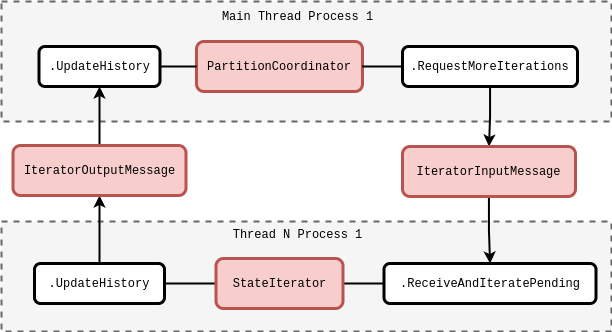
\includegraphics[width=10cm]{images/stochadex-loop.drawio.png}
\caption{Write software design diagrams}
\label{fig:loop-design}
\end{figure}


\chapter{\sffamily Simulating a financial market}

{\bfseries\sffamily Concept.} The idea here is to use the Q-Hawkes processes and the Bouchaud work to come up with some interesting simulations of financial markets. 

\section{\sffamily Introducing Q-Hawkes processes}


\chapter{\sffamily Quantum jumps on generic networks}

{\bfseries\sffamily Concept.} The idea is to follow this sort of thing \href{https://en.wikipedia.org/wiki/Quantum_jump_method}{here} to simulate the Lindblad equation over an arbitrary network of entangled states.

\section{\sffamily The Lindblad equation}


\part*{{\sffamily {\color{gray75} Part 2.} How do we then learn/identify the answer to Part 1 from real-world data?}}


\chapter{\sffamily Inferring dynamical 2D maps}

{\bfseries\sffamily Concept.} The idea here is 


\section{\sffamily Adapting the stochadex formalism}

\chapter{\sffamily Learning from ants on curved surfaces}

{\bfseries\sffamily Concept.} The idea here is 

\section{\sffamily Diffusive limits for ant interactions}


\chapter{\sffamily Hydrodynamic ensembles from input data}

{\bfseries\sffamily Concept.} The idea here is 


\section{\sffamily The Boltzmann/Navier-Stokes equations}

\chapter{\sffamily Generalised statistical inference tools}

{\bfseries\sffamily Concept.} The idea here is to extend the stochadex with tools for very generalised statistical inference (ABC algorithms and the like) that will work in nearly every situation. Probably need to exploit the phase space analogy of the formalism.

\section{\sffamily Likelihood-free methods}


\part*{{\sffamily {\color{gray75} Part 3.} How do we simulate a general set of control policies to interact with the answer to Part 1?}}


\chapter{\sffamily Interacting with systems in general}

{\bfseries\sffamily Concept.} The idea here is 

\section{\sffamily Parameterising general interactions}


\chapter{\sffamily Managing a Rugby match}

{\bfseries\sffamily Concept.} The idea here is 

\section{\sffamily Introduction}

Since the basic game engine will run using the \href{https://github.com/umbralcalc/stochadex}{stochadex} sampler, the novelties in this project are all in the design of the rugby match model itself. And, in this instance, I'm not especially keen on spending a lot of time doing detailed data analysis to come up with the most realistic values for the parameters that are dreamed up here. Even though this would also be interesting.

One could do this data analysis, for instance, by scraping player-level performance data from one of the excellent websites that collect live commentary data such as \href{https://www.rugbypass.com/}{rugbypass.com} or \href{https://www.espn.co.uk/rugby/}{espn.co.uk/rugby}.

This game is primarily a way of testing out the interface of the stochadex for other users to build projects with. This should help to both iron out some of the kinks in the design, as well as prioritise adding some more convenience methods for event-based modelling into its code base.

\section{\sffamily Designing the event simulation engine}

We need to begin by specifying an appropriate event space to live in when simulating a rugby match. It is important at this level that events are defined in quite broadly applicable terms, as it will define the state space available to our stochastic sampler and hence the simulated game will never be allowed to exist outside of it. So, in order to capture the fully detailed range of events that are possible in a real-world match, we will need to be a little imaginative in how we define certain gameplay elements when we move through the space.

The diagrams below sum up what should hopefully work as a decent initial approximation while providing a little context with specific examples of play action.

\begin{figure}[h]
\includegraphics[width=8cm]{images/test.drawio.png}
\caption{Simplified event graph of a rugby union match - replace with drawio.}
\label{fig:event-graph}
\end{figure}

\begin{figure}[h]
\includegraphics[width=10cm]{images/test.drawio.png}
\caption{Optional model ideas - replace with drawio.}
\label{fig:model-ideas}
\end{figure}

\section{\sffamily Linking to player attributes}

\section{\sffamily Deciding on gameplay actions}

\section{\sffamily Writing the game itself}

\chapter{\sffamily Influencing house prices}

{\bfseries\sffamily Concept.} The idea here is 


\part*{{\sffamily {\color{gray75} Part 4.} How do we then optimise the answer to Part 3 to achieve a specified control objective?}}


\chapter{\sffamily Optimising actions for control objectives}

{\bfseries\sffamily Concept.} The idea  controlhere is 


\chapter{\sffamily Resource allocation for epidemics}

{\bfseries\sffamily Concept.} The idea here is to limit the spread of some abstract epidemic through the correct time-dependent resource allocation.


\chapter{\sffamily Quantum system control}

{\bfseries\sffamily Concept.} The idea here is to follow stuff along these lines \href{https://arxiv.org/pdf/1210.7127.pdf}{here}.


\chapter{\sffamily Other models}

{\bfseries\sffamily Concept.} The idea here is




%\appendix
%\chapter{First and only appendix}
\backmatter
\bibliographystyle{JHEP}
\bibliography{book}
\end{document}